% ******** Приклад оформлення документа за ДСТУ 3008-95 ********
% ******************** автор: Тавров Д. Ю. *********************

% зазначаємо стильовий файл, який будемо використовувати
\documentclass{udstu}

% починаємо верстку документа
\begin{document}

% створимо титульний аркуш
% за допомогою спеціальної команди
% \maketitlepage{params},
% де params --- це розділені комами пари "параметр={значення}"
\maketitlepage{
% StudentName --- прізвище, ініціали студента
	StudentName={Скорденко Д. О.},
% StudentMale --- стать студента (true, якщо чоловік, false --- якщо жінка)
	StudentMale=true,
% StudentGroup --- група студента
	StudentGroup={КМ-01},
% Title --- назва
	Title={Звіт\\із лабораторної роботи №6\\із дисципліни \invcommas{Розподілені і хмарні обчислення}},
% SupervisorDegree --- науковий ступінь, учене звання керівника роботи
% якщо наукового ступеня немає, можна відповідний рядочок пропустити
	SupervisorDegree={доцент кафедри ПМА},
% SupervisorName --- прізвище, ініціали керівника роботи
	SupervisorName={Ліскін В. О.}
}

% створюємо зміст
\tableofcontents

% створюємо вступ
\intro

\paragraph{\textbf{Мета:}} створити програму для виділення областей зображення, та розпаралелити її.

Дослідний приклад:
\begin{equation*}
	A = \begin{bmatrix}
			1 & 1 & 0 & 0 & 0 & 0 \\
            1 & 1 & 0 & 1 & 0 & 0 \\
            1 & 0 & 0 & 0 & 0 & 0 \\
            0 & 0 & 1 & 1 & 1 & 1 \\
            1 & 0 & 0 & 1 & 0 & 0 \\
            1 & 0 & 0 & 1 & 0 & 1 \\
	    \end{bmatrix}
\end{equation*}


% створюємо перший розділ роботи
\chapter{Основна частина}
\label{chap:1}

\paragraph{\textbf{Опис програми:}}

Для реалізації паралелізму буде використовуватись 'Rayon'.
Для матриць / векторів буде використовуватись 'nalgebra'.

\chapter{Опис програми [Тестовий приклад]}
\label{chap:3}

\begin{figure}[!htp]
	\centering
	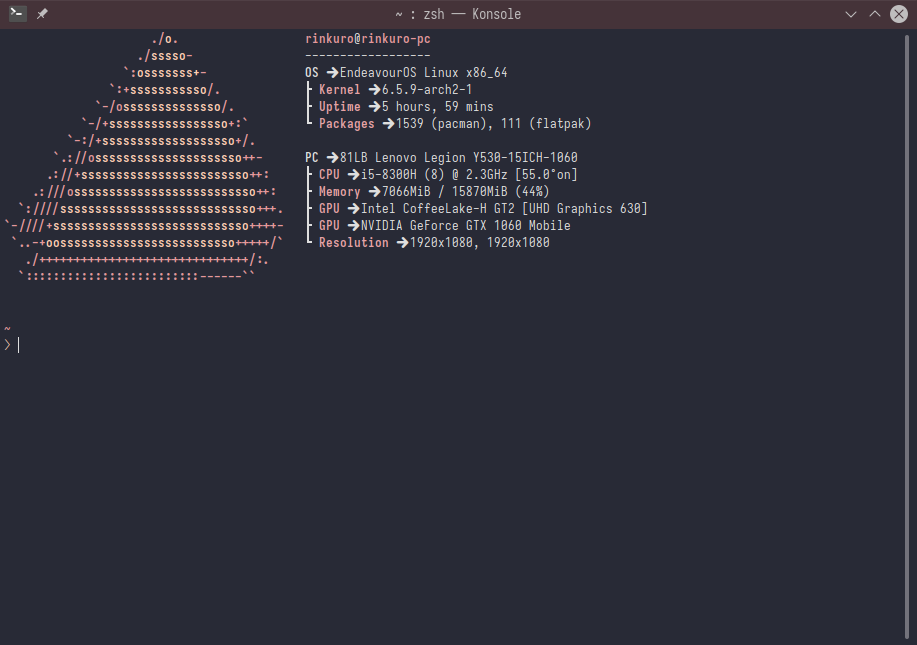
\includegraphics[scale=0.5]{PNG/system-specs.png}
	\caption{Характеристики системи}
	\label{fig:figure1}
\end{figure}

\begin{figure}[!htp]
	\centering
	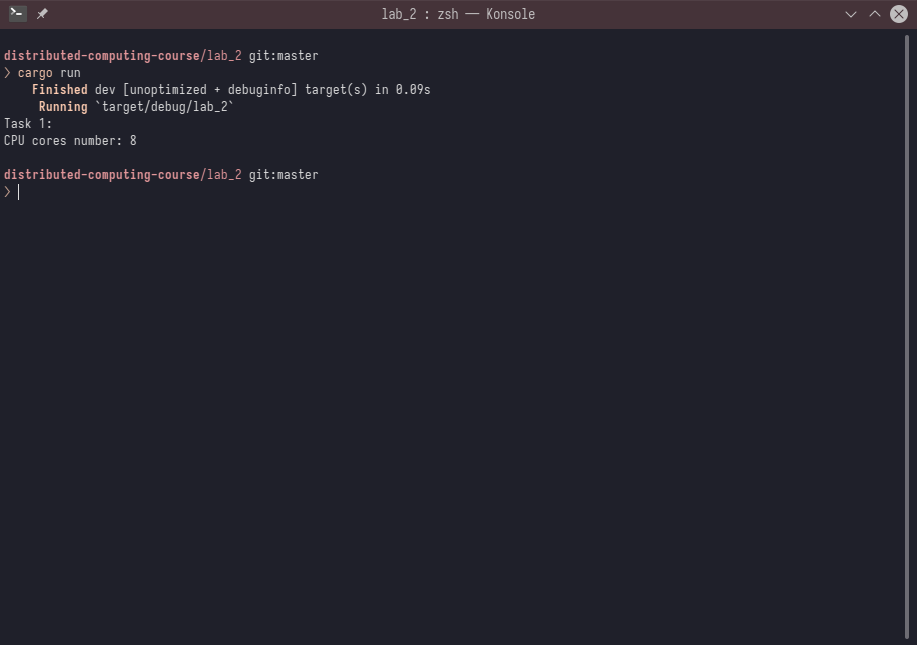
\includegraphics[scale=0.5]{PNG/thread-num-test.png}
	\caption{К-сть ядер процесора}
	\label{fig:figure1}
\end{figure}

\begin{figure}[!htp]
	\centering
	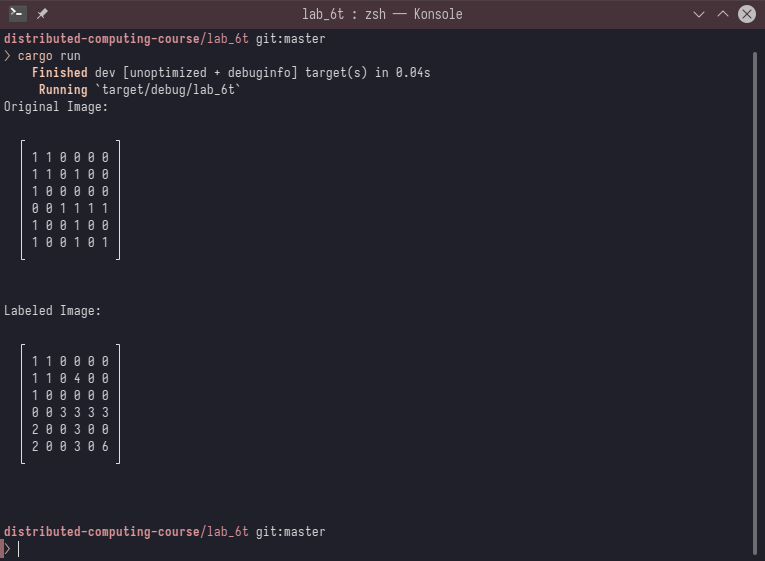
\includegraphics[scale=0.75]{PNG/test-case.png}
	\caption{Тестовий приклад}
	\label{fig:figure1}
\end{figure}

% створюємо Висновки
\conclusions

Було реалізовано виділення областей зображення у паралельному середовищі.

\append{Код лістінги}

\paragraph{\textsc{*Примітка:}}
У код лістингах при копіюванні втрачається форматування (не копіюються пробіли).
Файли прикріплено до цього pdf (вкладка "прикріплені файли").

\captionof{listing}{main.rs}
\embedfile[filespec=main.rs]{../src/main.rs}
\inputminted{rust}{../src/main.rs}

\end{document}
